\section{ToT 和 CoT 的对比}

\begin{frame}{ToT: 核心思想}
	\begin{figure}
        \centering
        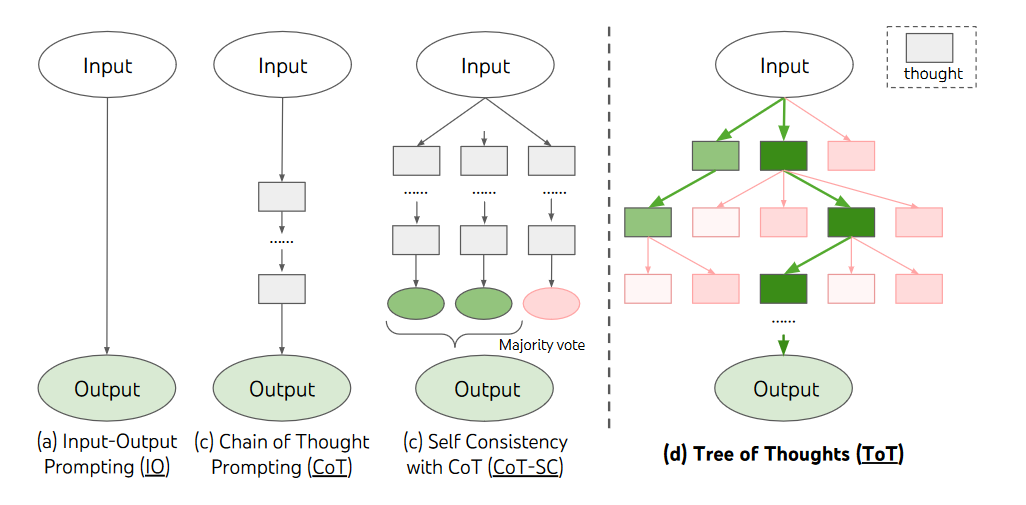
\includegraphics[width=.5\linewidth]{./pic/7.png}
    \end{figure}
\begin{itemize}
    \item ToT 将任何问题视为对一棵树的搜索。
    \item 每个节点表示一个状态 $ s = [x, z_{1 \cdots i}] $,即包含输入和当前思维序列的部分解决方案。
\end{itemize}
\end{frame}

\begin{frame}{ToT 的具体实现包括四个问题}
\begin{enumerate}
    \item 如何将中间过程分解为思维步骤;
	\bigskip
    \item 如何从每个状态生成潜在的思维;
	\bigskip
    \item 如何通过启发式方法评估状态;
	\bigskip
    \item 应该使用什么搜索算法。
\end{enumerate}
\end{frame}

\subsection{思维分解(Thought Decomposition)}

\begin{frame}{ToT 思维分解的核心思想}
\begin{itemize}
    \item 基于问题的特性设计并分解中间思维步骤。
	
    \bigskip
    \item 根据问题类型,“思维”的粒度可以灵活变化:
    \begin{itemize}
        \item 填字游戏:一个思维可能仅为几个单词。
        \item 24点游戏:一个思维可以是一行数学方程。
        \item 创意写作:一个思维可能是整段写作计划。
    \end{itemize}
\end{itemize}
\end{frame}

\begin{frame}{对思维粒度的要求}
\begin{itemize}
    \item 必须足够小:
    
    \begin{itemize}
        \item 以便 LM 能够生成多样且有希望的样本。
        
        \item 例如:生成一本书太大而无法连贯。
    \end{itemize}
	
	\pause
    \bigskip
    \item 必须足够大:
    
    \begin{itemize}
        \item 以便 LM 能够有效评估其在问题求解中的前景。
        
        \item 例如:生成一个 single token 太小而难以评估。
    \end{itemize}
\end{itemize}
\end{frame}

\subsection{思维生成器 $G(p_\theta, s, k)$}

\begin{frame}{思维生成器的设置}
\begin{itemize}
    \item 在树状态 $s = [x, z_{1 \cdots i}]$ 下,为生成下一个思维步骤的 $k$ 个候选项。
	\bigskip
    \item ToT 提供了两种生成策略。
\end{itemize}
\end{frame}

\begin{frame}{(a) 独立同分布采样(i.i.d.)}
\begin{itemize}
    \item 通过 CoT 提示生成 $k$ 个独立同分布的思维样本:
    \[
    z^{(j)} \sim p_\theta^{CoT}(z_{i+1} | s) = p_\theta^{CoT}(z_{i+1} | x, z_{1 \cdots i}), \ (j = 1 \cdots k).
    \]
	
	\pause
    \item 特点:
    \begin{itemize}
        \item 用于思维空间较丰富的场景(如创意写作)。
        \item 提升生成样本的多样性。
    \end{itemize}
\end{itemize}
\end{frame}
\begin{frame}{(a) 独立同分布采样(i.i.d.)}
\begin{figure}
	\centering
	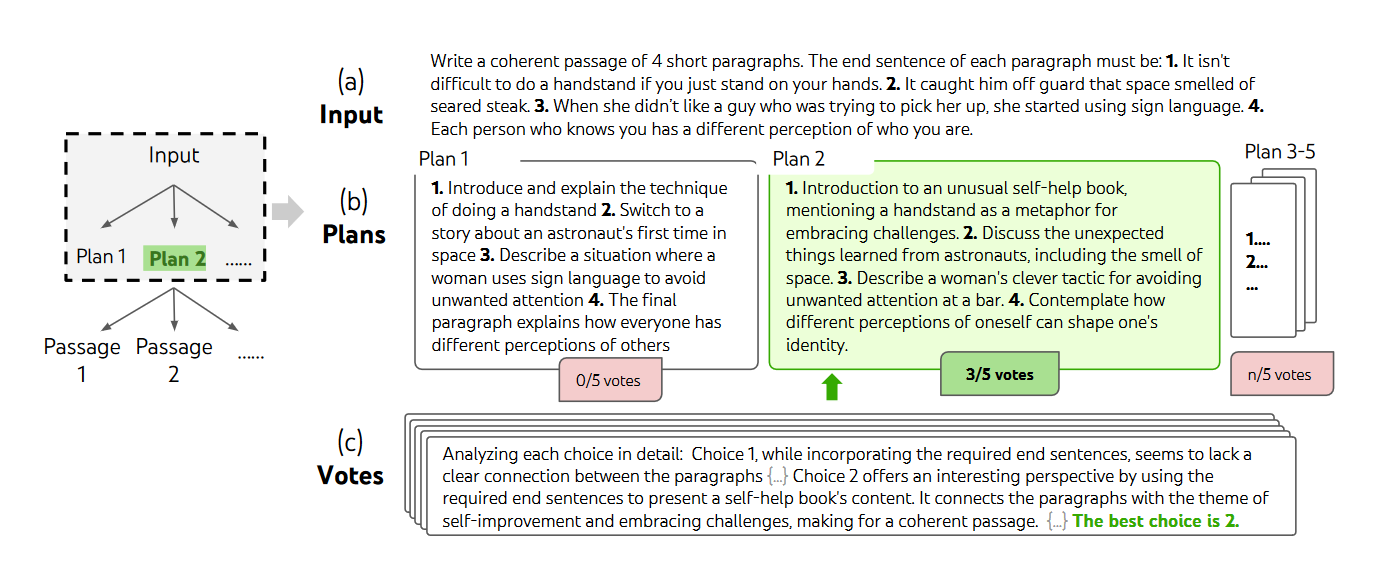
\includegraphics[width=.9\linewidth]{./pic/8.png}
	\caption{独立同分布采样示例,创意写作}
\end{figure}
\end{frame}

\begin{frame}{(b) 顺序提示}
\begin{itemize}
    \item 按顺序生成 $k$ 个思维候选项:
    \[
    [z^{(1)}, \cdots, z^{(k)}] \sim p_\theta^{propose}(z_{i+1}^{(1 \cdots k)} \mid s).
    \]
	
	\pause
    \bigskip
    \item 特点:
    \begin{itemize}
        \item 适用于思维空间较为有限的场景。
        \item 例如:24点游戏或填字游戏(每个思维为一个单词/方程)。
    \end{itemize}
\end{itemize}
\end{frame}

% \begin{frame}{示例}
% \centering
% \includegraphics[width=0.8\textwidth]{https://raw.githubusercontent.com/Lanthanum1/my_images/main/img/202412052048081.png}
% \end{frame}

\subsection{状态评估器 $V(p_\theta, S)$}

\begin{frame}{状态评估器的功能}
\begin{itemize}
    \item 对一组边界状态 $S$ 进行评估,衡量其在解决问题上的进展。
	\bigskip
    \item LM 通过推理提供启发,以确定需要继续探索的状态及其顺序。
	\bigskip
    \item 与传统启发式方法相比:
    \begin{itemize}
        \item 比硬编码更灵活。
        \item 比学习模型高效(尤其在样本有限下)。
    \end{itemize}
\end{itemize}
\end{frame}

\begin{frame}{状态评估策略}
\begin{itemize}
    \item (a) 独立评估每个状态
    \[
    V(p_\theta, S)(s) \sim p_\theta^{\text{value}}(v \mid s), \quad \forall s \in S.
    \]
	
	\pause
    \item (b) 跨状态投票
    \[
    s^* \sim p_\theta^{\text{vote}}(s^* \mid S).
    \]
\end{itemize}
\end{frame}

\begin{frame}{(a) 独立评估每个状态}
\begin{itemize}
    \item 前瞻模拟:
    \begin{itemize}
        \item 验证状态是否有潜力。
        \item 例如:数字组合是否能达到目标。
	
	\pause
    \end{itemize}

    \bigskip
    \item 常识判断:
    \begin{itemize}
        \item 排除明显错误的状态。
        \item 例如:“tzxc”不可能构成单词。
    \end{itemize}
\end{itemize}
\end{frame}

\begin{frame}{(b) 跨状态投票}
\begin{itemize}
    \item 比较各状态,投票选择最优状态。
	\bigskip
    \item 对多选问题的多次采样结果进行比较。
	\bigskip
    \item 示例:文章段落的连贯性。
\end{itemize}
\end{frame}

\subsection{搜索算法}

\begin{frame}{搜索算法}
\begin{itemize}
    \item 论文实现了 BFS 和 DFS。
    \item Leaving more advanced ones (e.g. A* [11], MCTS [2]) for future work。
\end{itemize}
\begin{figure}
	\centering
	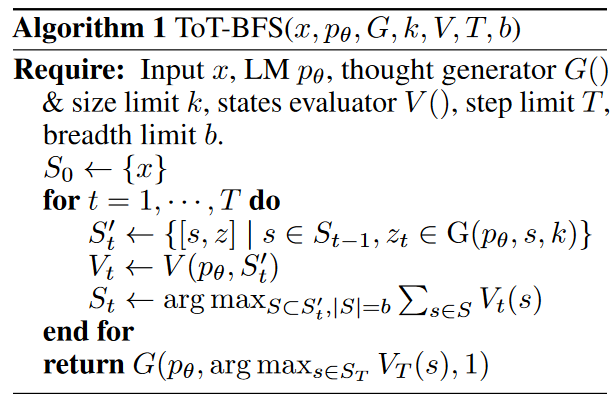
\includegraphics[width=.5\linewidth]{./pic/9.png}
\end{figure}
\end{frame}

\begin{frame}{BFS 搜索策略}
每一步维护 $b$ 个最佳候选项:
\begin{itemize}
    \item 提取剩余数字并提示语言模型生成候选。
    \item 对每个候选项进行评估(例如:是否能达到目标)。
    \item 选择前 $b$ 个部分解继续搜索。
\end{itemize}
\begin{figure}
	\centering
	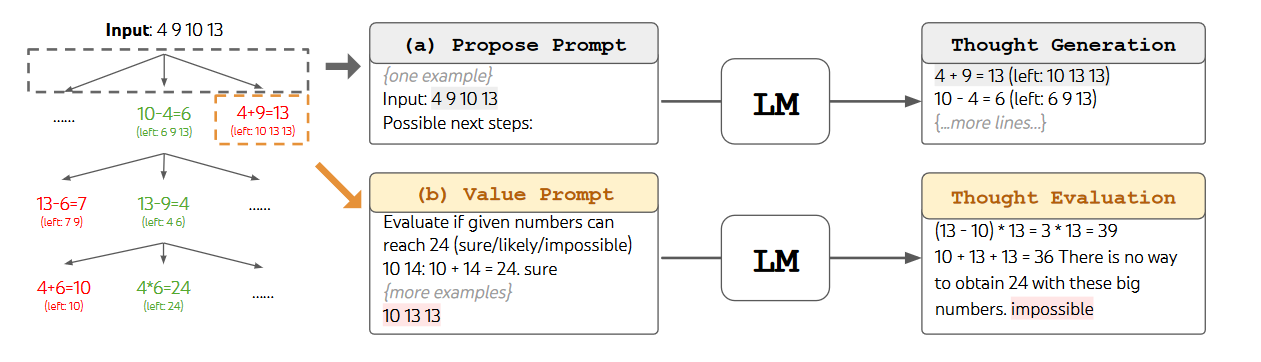
\includegraphics[width=.8\linewidth]{./pic/10.png}
	\caption{BFS 搜索示例,24 点}
\end{figure}
\end{frame}

\begin{frame}{DFS 搜索策略}
\begin{itemize}
    \item 优先搜索当前最佳状态。
    \item 如果状态评估器判断当前状态不可行:
    \begin{itemize}
        \item 剪枝该状态的子树。
        \item 回溯到父节点。
    \end{itemize}
\end{itemize}
\begin{figure}
	\centering
	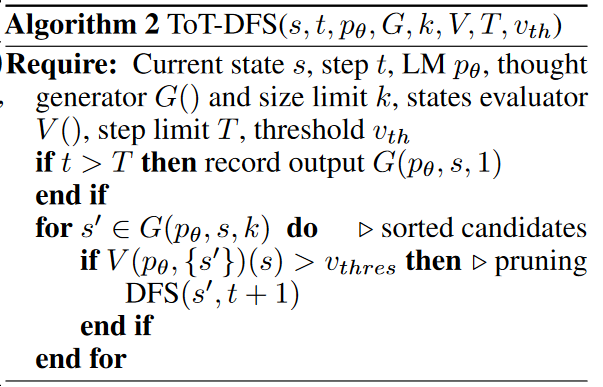
\includegraphics[width=.5\linewidth]{./pic/11.png}
\end{figure}
\end{frame}